\chapter{Divide Areas Algorithm}
\label{chp:DARP}

%%%%%%%%%%%%%%%%%%%%%%%%%%%%%%%%%%%%%%%%%%%%%%%%%%%%%%%%%%%%%%%%%%%%%%%
\section{Background}
The research aim in section \ref{sec:intro_researchAim} refers to the development of a coverage path planning algorithm using multiple UAVs. Coverage path planning is often linked to applications such as surveying, mapping and searching, because it involves planning a UAVs path so as to cover all points in an environment. The idea is then that one could speed up the time taken to cover the environment mentioned by using several UAVs searching in tandem.

Before one can begin covering an area, the points within this area that must be searched require identifying. With coverage path planning, grid-based methods are quite popular because they make it easy to divide an area into searchable cells.
% TODO: Include more justification on grid based
Grid-based coverage path planning can be implemented using a number of different methods. 

Naturally, achieving the most optimal solution possible would be most desirable. The authors of \cite{DARP2017} propose a set of requirements for optimal coverage path planning using a grid-based approach. These fundamental conditions, as they call them, are listed below.

\begin{enumerate}
	\item Every cell in the environment, that is not classified as an object, must be covered. This is known as complete coverage.
	\item Each cell in the environment must only be searched once, and only by one of the robots. This is known as the non-backtracking requirement.
	\item Each robot should have as close to an equal amount of cells as possible assigned to it for searching. Their sets of cells should be of roughly the same size.
	\item The sets of cells assigned to each robot should be a connected sub-region. This means that when generating a path to search the cells within its set, a robot would not need to traverse that of another to search it's own sub-region.
	\item The initial position of each robot should be contained within the set of cells assigned to it. This means that a robot would not need to travel to reach its sub-region for searching.
\end{enumerate}
% TODO: Maybe mention something about the EXISTENCE of solutions
% Coverage
% Grid Based
% Optimize

\begin{figure}[h!]
	\centering
	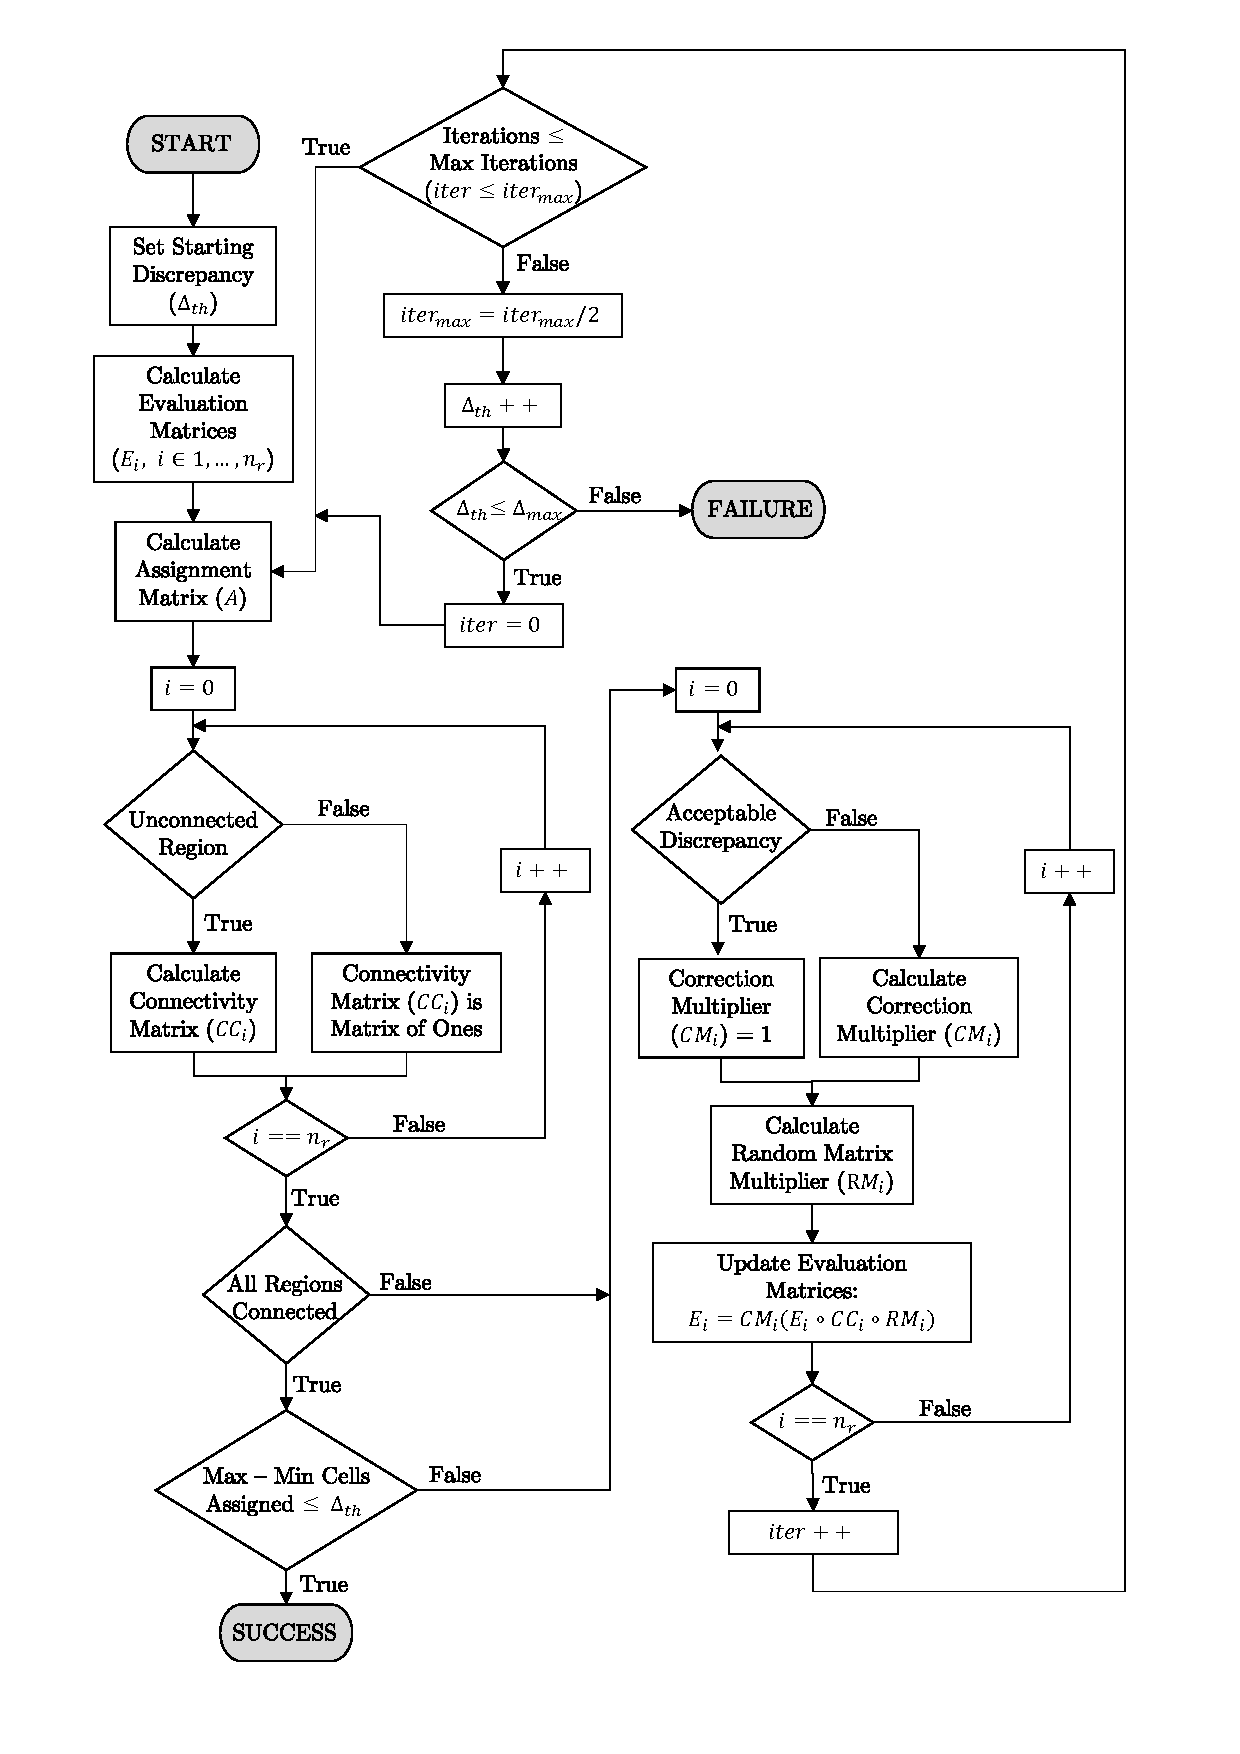
\includegraphics[scale=0.8,trim={1.5cm 0 1.5cm 0},clip]{figs/DARP_Diagram3.pdf}
	\caption{}
	\label{fig:DARP}
\end{figure}

%%%%%%%%%%%%%%%%%%%%%%%%%%%%%%%%%%%%%%%%%%%%%%%%%%%%%%%%%%%%%%%%%%%%%%%
\section{Implementation}
\subsection{Comparison of Distance Measures}
